\documentclass[12pt,letterpaper]{extreport}
\usepackage[12pt]{extsizes}
\usepackage[utf8]{inputenc}
\usepackage[russian]{babel}
\usepackage[OT1]{fontenc}
\usepackage{amsmath}
\usepackage{amsfonts}
\usepackage{amssymb}
\usepackage{graphicx}
\usepackage{geometry}
\usepackage{wrapfig}
\usepackage{float}
\usepackage{caption}
\RequirePackage[
  		a4paper, mag=1000,
  		left=2.5cm, right=1.5cm, top=2cm, bottom=2cm, bindingoffset=0cm,
		headheight=0cm, footskip=1cm, headsep=0cm
	]{geometry}

\begin{document}
\pagestyle{empty}

\begin{flushright}
{\bfseries \large УДК 539.3}
\end{flushright}

\begin{center}
\textbf{Вычислительный эксперимент пологих, гибких прямоугольных в плане
оболочек}\\
Иванов И.И., Петров П.П., Федоров Ф.Ф.\\
\textit{adress@email.ru}\\
\end{center}

\textbf{Введение:\\
1.	Основные уравнения}
\par Для интегрирования уравнений в частных производных используется метод
конечных разностей с аппроксимацией $O(h2)$ как по временной, так и по
пространственной координате. 
\par Для этого область $D=\left\{(x,t)|0\leq x \leq 1 , 0 \leq t \leq T\}
\right. $  покрывалась прямоугольной сеткой  , где $x_i =x_{i+1} -
x_i=h_x=1/n_x$  ($n_x$  целое) и $h_t=t_{j+1}-t_j$ . $h_z =1.0/h_z$ .
На сетке дифференциальные уравнения приближенно заменяются соответствующими
конечно-разностными соотношениями. С целью повышения точности использовались
симметричные формулы для производных. После несложных преобразований 
получаем\\
$w_{li, j+1}=\frac{1}{1+\varepsilon_l h_t /2b_l h_l} \left[2w_{li,j}+
(\frac{\varepsilon_l h_t}{2h_l}-1)w_{li,j-1}+\frac{h_t^2}{b_l h_l}A_{li,j}
\right],$
\\$u_{ij+1}=\frac{h_t^2}{bh}
\left[\frac{\partial E_{0l}}{\partial
x}(u'+\frac{1}{2}(w')^2)+E_{0l}(u"+w'w'')-\frac{\partial E_{1l}}{\partial x}w''
- E_{1l}w'''

\right]_{ij} +2u_{ij},$\\
\par гдe\\
$A_{li,j}=\frac{\partial^2}{\partial x^2}\left[E_{1l}(u'_l +
\frac{1}{2}(w'_l)^2)-E_{2l}w'''\right] -\frac{\partial}{\partial
x}\left[w'E_{0l}(u'_l
+\frac{1}{2}(w'_l)^2)-E_{1l}w''\right]_{i,j}$\\

\par Начальные условия:

$w_{l-1,j} - 2w_{l0,j} + w_{l1,j} = 0, w_{l0,j} = 0, w_{ln-1,j} - 2w_{in,j} + 
w_{ln+1,j} = 0,
w_{ln,j} =0; u_{l0, j}= u_{ln,j} = 0, $

\par Граничные условия:

$\frac{w_{li,j+1} -w_{li,j}}{h_t}=F_{li}, w_{li} = f_{li}, u_{li} = u_{l0i}, $
     
\par Установлено, что для получения результатов с необходимой степенью точности
в МКР
достаточно
разбить интервал интегрирования [0,1] на 40 частей. [3] На каждом шаге по 
времени строится итерационная процедура метода переменных параметров упругости 
Биргера. 

\par \textbf{Результаты и их анализ}\\
Полученный в данном эксперименте сценарий очень интересен, т. к. появление 
независимой частоты здесь приводит не к жесткому переходу колебаний оболочки в 
хаотические, а к бифуркации утроения периода. Утроение периода колебаний 
происходит резко не только с увеличением амплитуды сдвиговой силы, но при ее  
фиксированном значении с течением времени. Дальнейший переход сисчтемы к хаосу 
осуществляется через перемежаемость. Т. е. при движении по амплитуде нагрузки 
возникает все большее количество хаотических зон, мало того их расположение на 
вейвлет спектре имеет периодический характер. Таким образом с ростом 
управляющего параметра не только увеличевается количество окон хаоса, но и 
сокращается период их появления. 

\par Данный сценарий можно назвать модифицированным сценарием Помо – Манневиля 
(модификации
2).

\begin{table}[H]

{\setlength{\arrayrulewidth}{1.25pt}
\begin{flushright}
Таблица 7\\
Характеристики оболочки $k_x=k_y=12$ , $\omega_p= \omega_0 =11.4$, $s_0=15.726$
на различных временных интервалах.

\end{flushright}
\begin{tabular}{|c|c|c|c|}

\hline
\multicolumn{4}{|c|}{А. Характеристики оболочки t $\in$ [30,109]}

\\
\hline
\footnotesize 2-D Вейвлет спектр Морле&\footnotesize Фазовый 
портрет&\footnotesize 3D
Модальный
портрет 3D&\footnotesize Спектр мощности\\
\hline
	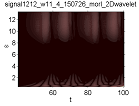
\includegraphics[scale=1]{a1} 	
	&	
	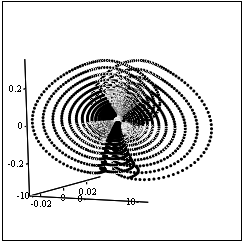
\includegraphics[scale=1]{a2} 	
	&	
	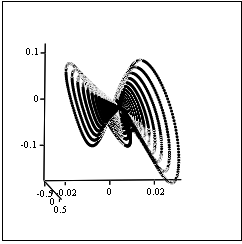
\includegraphics[scale=1]{a3} 
	&
	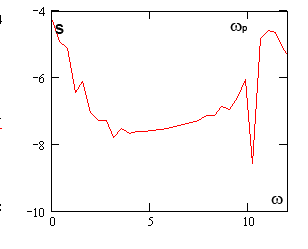
\includegraphics[scale=1]{a4} 
\\
\hline
\multicolumn{4}{|c|}{В. Характеристики оболочки t $\in$ [30,46]}\\

\hline
\footnotesize 2-D Вейвлет спектр Морле&\footnotesize Фазовый 
портрет&\footnotesize 3D Модальный портрет 3D&\footnotesize Спектр мощности\\
\hline
	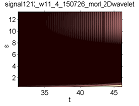
\includegraphics[scale=1]{b1} 	
	&	
	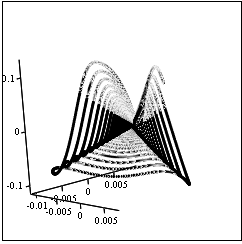
\includegraphics[scale=0.9]{b2} 	
	&	
	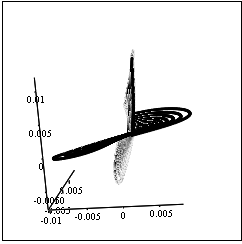
\includegraphics[scale=0.9]{b3} 
	&
	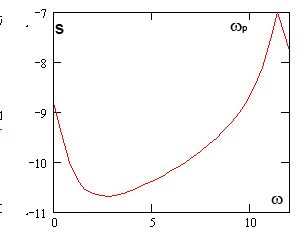
\includegraphics[scale=0.9]{b4} 
\\
\hline

\multicolumn{4}{|c|}{С. Характеристики оболочки  t $\in$ [50,66]}\\

\hline
\footnotesize 2-D Вейвлет спектр Морле&\footnotesize Фазовый 
портрет&\footnotesize 3D Модальный портрет 3D&\footnotesize Спектр мощности\\
\hline
	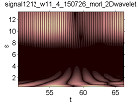
\includegraphics[scale=1]{c1} 	
	&	
	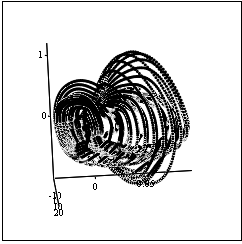
\includegraphics[scale=0.9]{c2} 	
	&	
	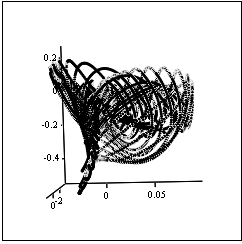
\includegraphics[scale=0.9]{c3} 
	&
	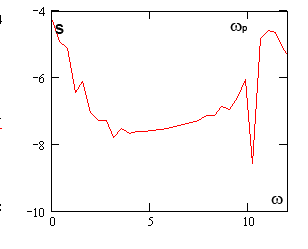
\includegraphics[scale=0.9]{c4} 
\\
\hline

\multicolumn{4}{|c|}{D. Характеристики оболочки t  t $\in$ [110,126]}\\

\hline
\footnotesize 2-D Вейвлет спектр Морле&\footnotesize Фазовый 
портрет&\footnotesize 3D Модальный портрет 3D&\footnotesize Спектр мощности\\
\hline
	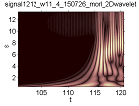
\includegraphics[scale=1]{d1} 	
	&	
	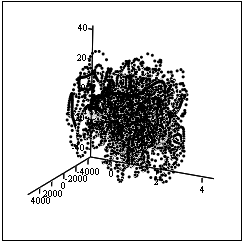
\includegraphics[scale=0.9]{d2} 	
	&	
	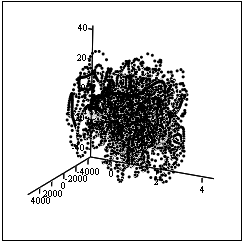
\includegraphics[scale=0.9]{d3} 
	&
	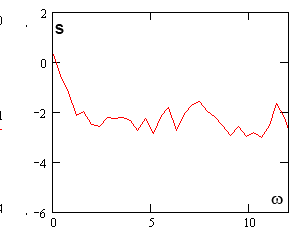
\includegraphics[scale=0.9]{d4} 
\\
\hline

\multicolumn{4}{|c|}{E. Характеристики оболочки  t $\in$ [130,258]}\\

\hline
\footnotesize 2-D Вейвлет спектр Морле&\footnotesize Фазовый 
портрет&\footnotesize 3D Модальный портрет 3D&\footnotesize Спектр мощности\\
\hline
	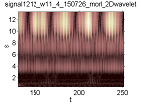
\includegraphics[scale=0.9]{e1} 	
	&	
	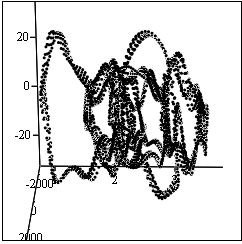
\includegraphics[scale=0.9]{e2} 	
	&	
	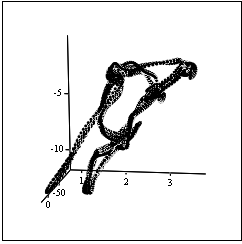
\includegraphics[scale=0.9]{e3} 
	&
	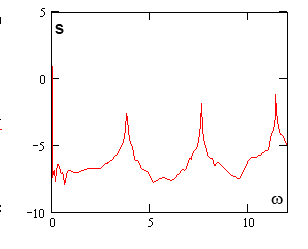
\includegraphics[scale=0.9]{e4} 
\\
\hline
\end{tabular}

}
\end{table}	
\par Было выяснено, что математический аппарат быстрого преобразования Фурье не
позволяет в полной мере проанализировать характер подобных колебаний и 
построить, как это традиционно делалось, сценарии перехода системы в хаос. По 
этому в работе поведение оболочек исследовалось на основании вейвлет анализа.

\par Трехмерный Вейвлет спектр указывает на то, что хаос наступает на низких 
частотах.

\begin{center}
\begin{figure}
\centering
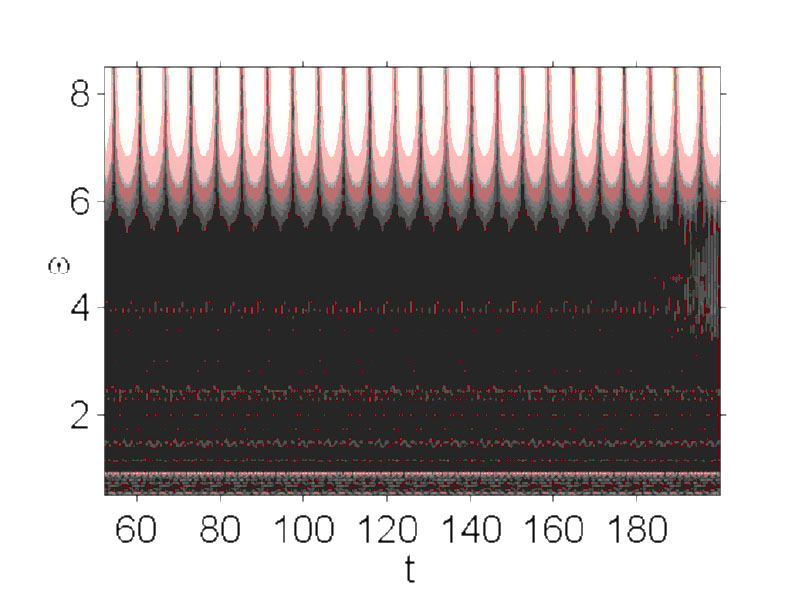
\includegraphics[scale=0.5]{ris5}
\end{figure}
Рис 5. Вейвлет спектр на интервале $52\leq t \leq 200, s_0=18.7, \omega_p = 
8.7.$
\end{center}

\par По средствам вейвлет анализа было выяснено, что характер колебаний 
оболочки под действием внешней знакопеременной сдвиговой нагрузки, с течением 
времени, может меняться от гармонического и квазипериодического до хаотического
при постоянных значениях амплитуды и частоты воздействия. Также могут 
наблюдаться кратковременные области хаотических колебаний
внутри квазипериодического окна и квазипериодические зоны внутри гармонических 
областей. Таким образом, происходит потеря устойчивости системы не только при 
изменении некоторых управляющих параметров, но и при их фиксированных значениях
с течением времени, т. е. наблюдается перемежаемость по времени.

\par В результате численных экспериментов установлено, что единого сценария
перехода в хаос для рассматриваемых систем нет. В зависимости от геометрических
параметров оболочки и частоты внешней знакопеременной сдвиговой нагрузки
сценарии существенно меняются. Было получено несколько сценариев большая часть
из которых - новые: сценарий Фейгенбаума (и посчитана константа Фейгенбаума),
сценарии Помо – Манневиля трех различных модификаций, сценарии Рюеля - Такенса
- Ньюхауся четырех различных модификаций и принципиально новый сценарий 
(ПНС).\\

\leftline{\textbf{Литература}}

\begin{enumerate}

\item \textbf{Krysko V.A., Awrejcewicz J., Bruk V.M.} On the solution of a
coupled thermo-mechanical problem for non-homogeneous Timoshenko-type shells //
Journal of Mathematical Analysis and Applications.2003. № 273. P. 409-416.

\item \textbf{Krysko V.A., Awrejcewicz J., Bruk V.M.} On existence and 
uniqueness of solutions to coupled thermomechanics problem of non- homogeneous
isotropic plates // J. Appl. Anal. 2002. № 8(1). P. 129 – 139.

\item \textbf{Вольмир А.С.} Устойчивость упругих систем. М.: Физматгиз, 1963,
880 с.

\item \textbf{Awrejcewicz J., Krysko V., Narkaitis G.} Bifurcations of Thin
Plate – Strip Excited Transversally and Axially. Nonlinear Dynamics, 32, p. 187
- 209, 2003.

\end{enumerate}

\end{document}